\documentclass[11pt]{article}
\usepackage{xeCJK}
\usepackage[a4paper, margin=1.4in]{geometry}
\usepackage{fancyhdr}
\usepackage{graphicx}
\usepackage{framed} 

\linespread{1.25}
\setlength\parindent{0pt}

\title{%
  \LARGE
  \textbf{COMP90086 Computer Vision \\
  \large Week 2B
  \\
  Image Filtering - Frequency Filtering}}
\author{ Lecture Notes summarized by Neo }
\date{Semester 2 2021}

\pagestyle{fancy}
\fancyhf{}
\rhead{COMP90086 Computer Vision}
\lhead{Lecture Notes}
\rfoot{Page \thepage}

\begin{document}

\maketitle


\section{Fourier Analysis (1D)}

\subsection{Signals 信号}
Any signal or pattern can be described as a sum of sinusoids.
所有信号都可以表示成很多正弦函数的叠加(和)。
\begin{figure}[bht!]
  \centering
  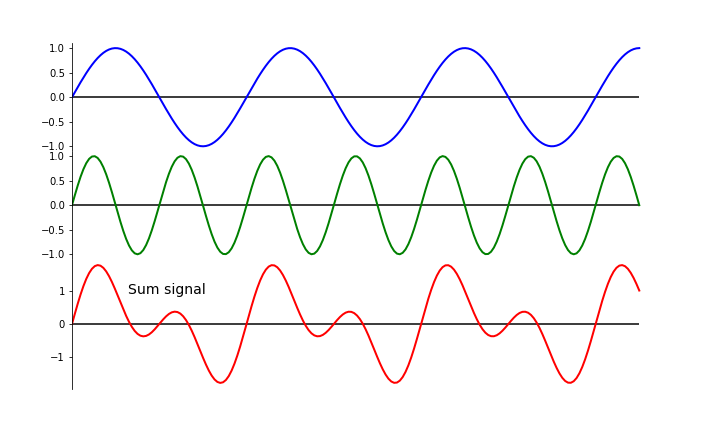
\includegraphics[width=\textwidth]{images/signals.png}
\end{figure}
\begin{itemize}
  \item 红色的复杂信号,可以分解成蓝色正弦函数信号与绿色正弦函数的叠加
  \item \textbf{一张图片上截取一行Pixel,可以转换成一段信号,所以叫1D}
\end{itemize}

\newpage
\subsection{Sinusoids (Sine Waves) 正弦函数}
$$y=A\sin (wx+\varphi )$$
where
\begin{itemize}
  \item $A$ is amplitude
  \item $w$ is frequency
  \item $\varphi$ is phase
\end{itemize}

\subsection{Fourier Transform 傅里叶变换}
Fourier transform decomposes signal into component frequencies.\\
傅里叶变换是一种线性积分变换,用于信号在时域(或空域)和频域之间的变换。

\begin{figure}[bht!]
  \centering
  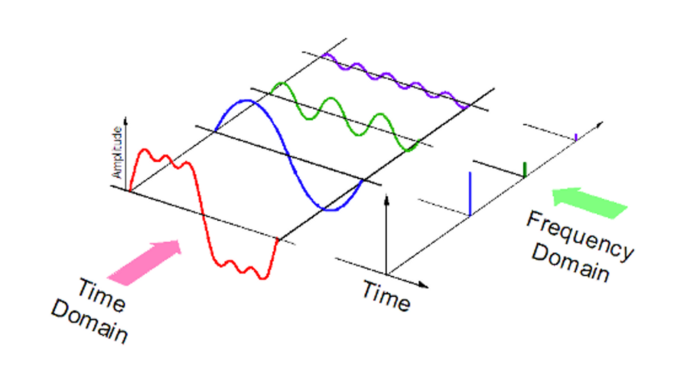
\includegraphics[width=\textwidth]{images/fourier.png}
\end{figure}

\begin{figure}[bht!]
  \centering
  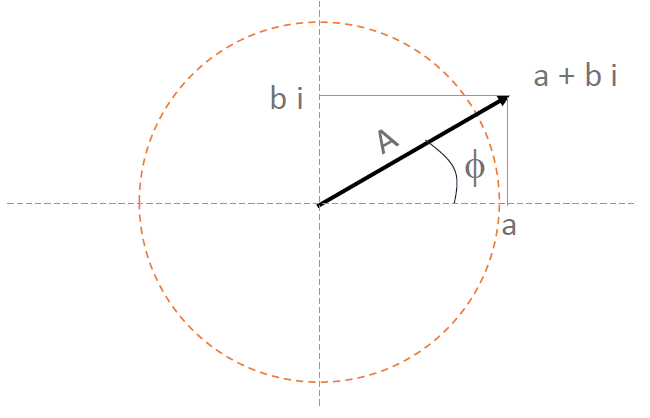
\includegraphics[width=0.6\textwidth]{images/angle.png}
\end{figure}

\begin{itemize}
  \item Frequency Domain:
        \begin{itemize}
          \item The axis is frequency
          \item Values are complex numbers
          \item Magnitude = amplitude of the sinusoid
          \item Angle = phase of the sinusoid
        \end{itemize}
\end{itemize}


\subsubsection*{Formula (Not assessable)}
$$F(w)=\int_{-\infty}^{\infty}f(x)e^{-2i\pi wx} dx$$
一般有包可以直接用,例如scipy.fft(1D), scipy.fft2(2D), scipy.fftn(3D+)



\section{Fourier Analysis (Image 2D)}
\begin{framed}
  \begin{center}
    在2D图像中,x轴与y轴可分别做傅里叶变换并放到右图以0freq为中心的轴中。
  \end{center}
\end{framed}
\begin{figure}[bht!]
  \centering
  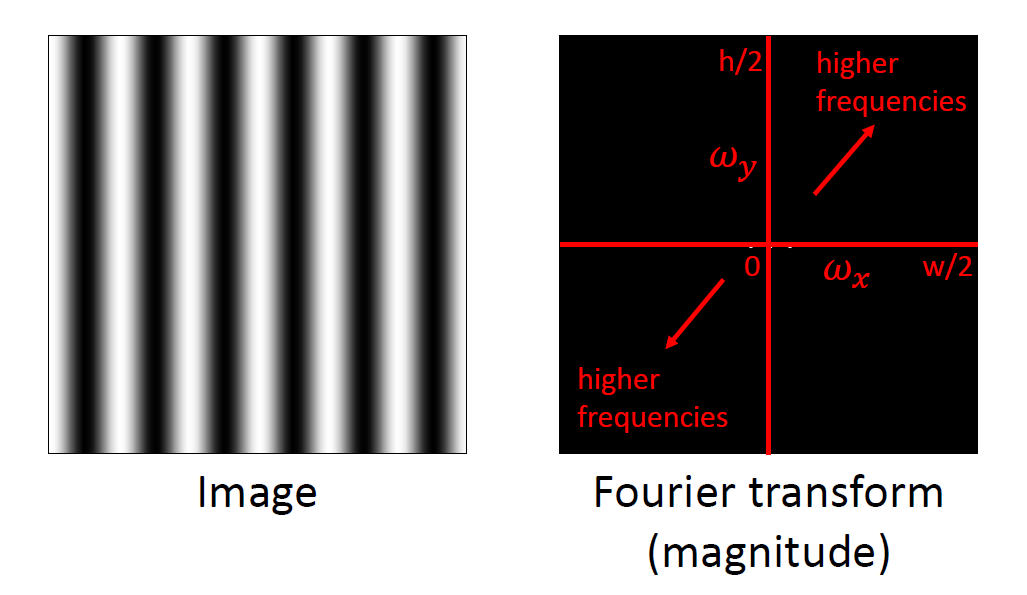
\includegraphics[width=\textwidth]{images/2d.png}
\end{figure}
\begin{framed}
  \begin{center}
    频率图中坐标表示不同的频率,白点的亮度代表频率的大小。
  \end{center}
\end{framed}

\newpage
\subsection*{Examples}
\begin{itemize}
  \item 只有横坐标有frequency
\end{itemize}
\begin{figure}[bht!]
  \centering
  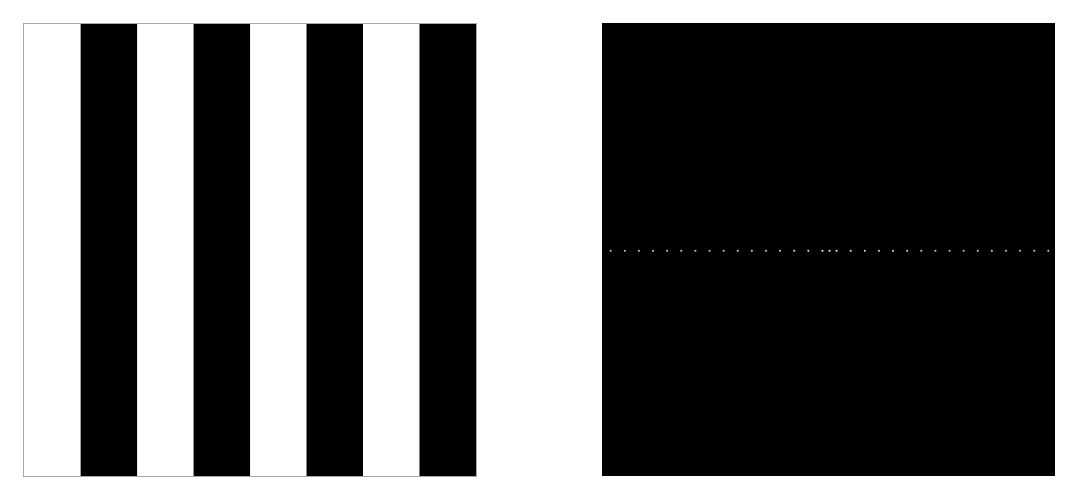
\includegraphics[width=0.8\textwidth]{images/e1.png}
\end{figure}
\begin{itemize}
  \item 横竖坐标都有frequency
\end{itemize}
\begin{figure}[bht!]
  \centering
  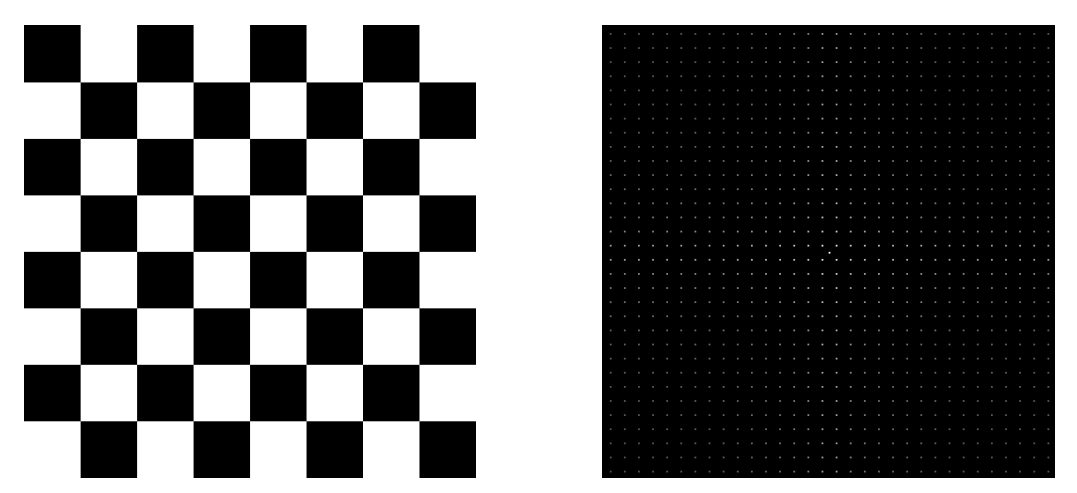
\includegraphics[width=0.8\textwidth]{images/e2.png}
\end{figure}
\begin{itemize}
  \item 真实的图片(大部分图片都类似,会有很多非常低的频率出现)
\end{itemize}
\begin{figure}[bht!]
  \centering
  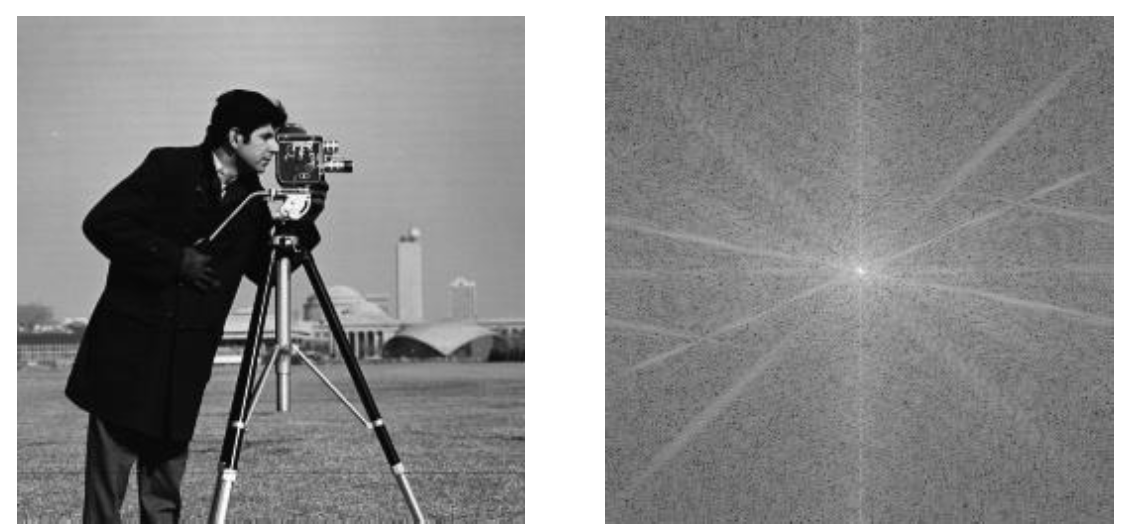
\includegraphics[width=0.87\textwidth]{images/e3.png}
\end{figure}

\subsection{Magnitude and Phase}
\begin{figure}[bht!]
  \centering
  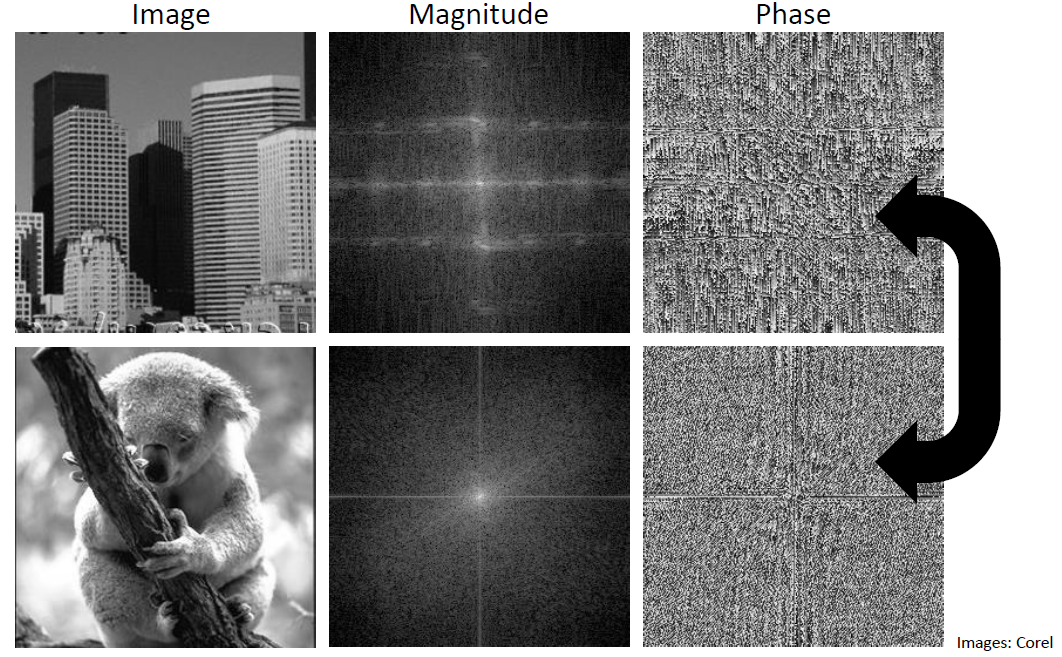
\includegraphics[width=\textwidth]{images/magnpha.png}
\end{figure}
\begin{figure}[bht!]
  \centering
  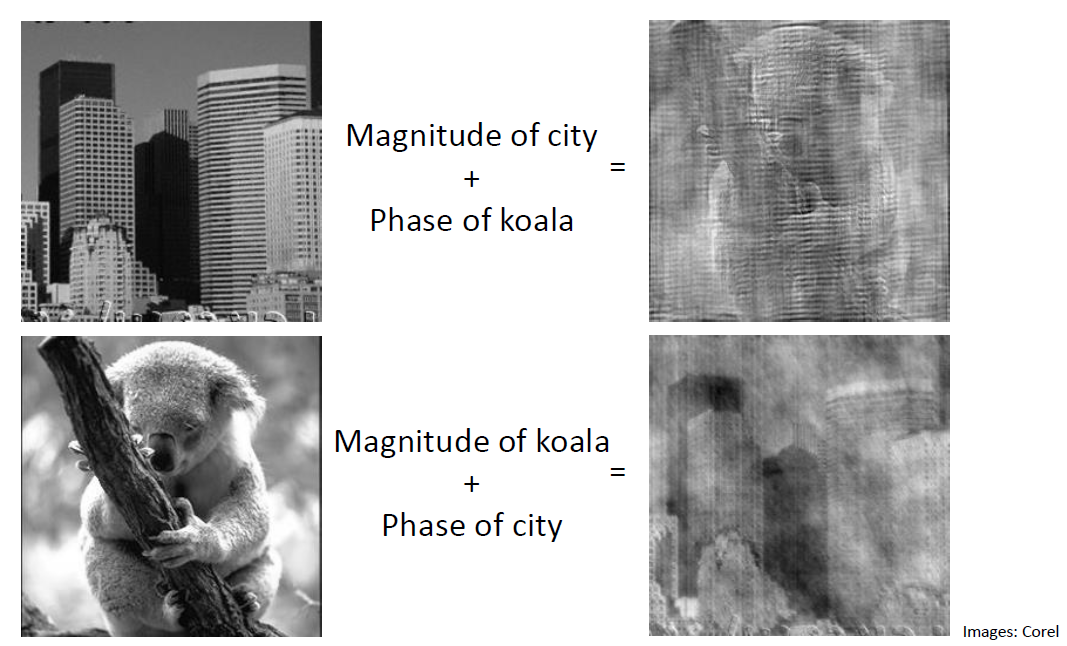
\includegraphics[width=\textwidth]{images/magnpha2.png}
\end{figure}
\begin{itemize}
  \item Any image can be represented by its Fourier transform
  \item Fourier transform = for each frequency, magnitude (amplitude) + phase
  \item Magnitude captures the holistic “texture” of an image, but the edges are mainly represented by Fourier phase
\end{itemize}

\section{Frequency Filtering}
Operations in the spatial domain have equivalent operations in frequency domain\\
每个在空域的操作都有对应在频域的操作。
\begin{framed}
  \begin{center}
    Convolution in spatial domain = multiplication in frequency domain\\
    空域卷积$=$频域相乘
  \end{center}
\end{framed}

\subsection{Bandpass Filter}
A filter that removes a range of frequencies from a signal.

\subsection{Low Pass Filter}
Keep low spatial frequencies, remove high frequencies.
\begin{figure}[bht!]
  \centering
  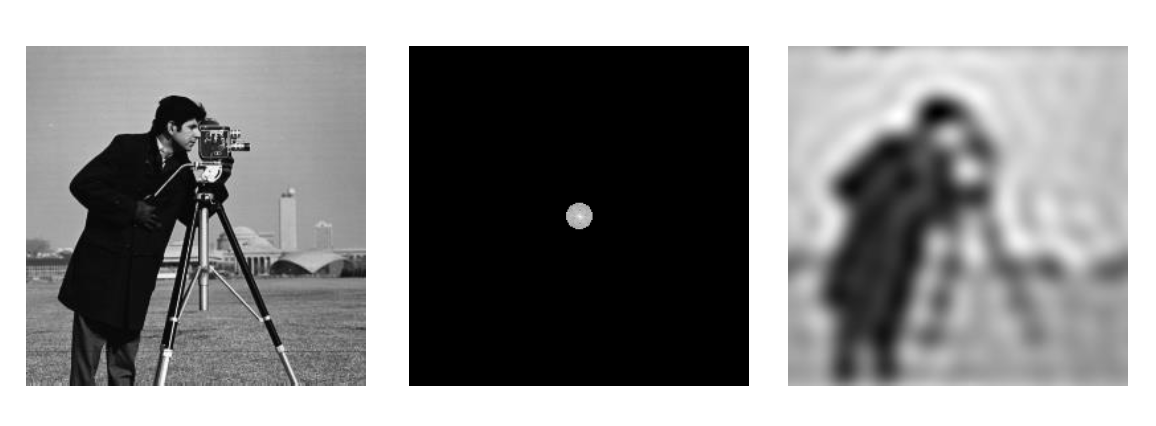
\includegraphics[width=\textwidth]{images/lowpass.png}
\end{figure}

\subsection{High Pass Filter}
Keep high spatial frequencies, remove low frequencies.
\begin{figure}[bht!]
  \centering
  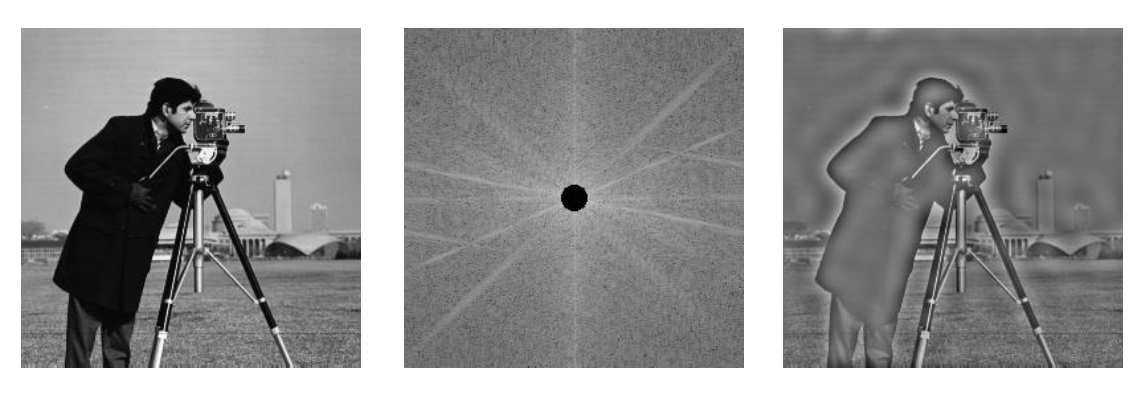
\includegraphics[width=\textwidth]{images/highpass.png}
\end{figure}

\subsection{Filter Artefacts}
\begin{figure}[bht!]
  \centering
  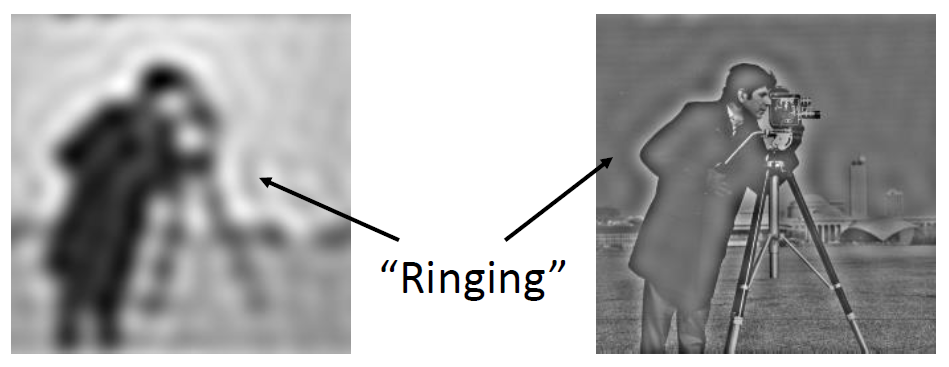
\includegraphics[width=\textwidth]{images/art.png}
\end{figure}
\begin{framed}
  \begin{center}
    我们会发现直接使用Low/High Pass的效果并不好,会使图片出现水滴状的效果,原因是因为没有使用“圆滑”的filter。
  \end{center}
\end{framed}
What we are doing:
\begin{figure}[bht!]
  \centering
  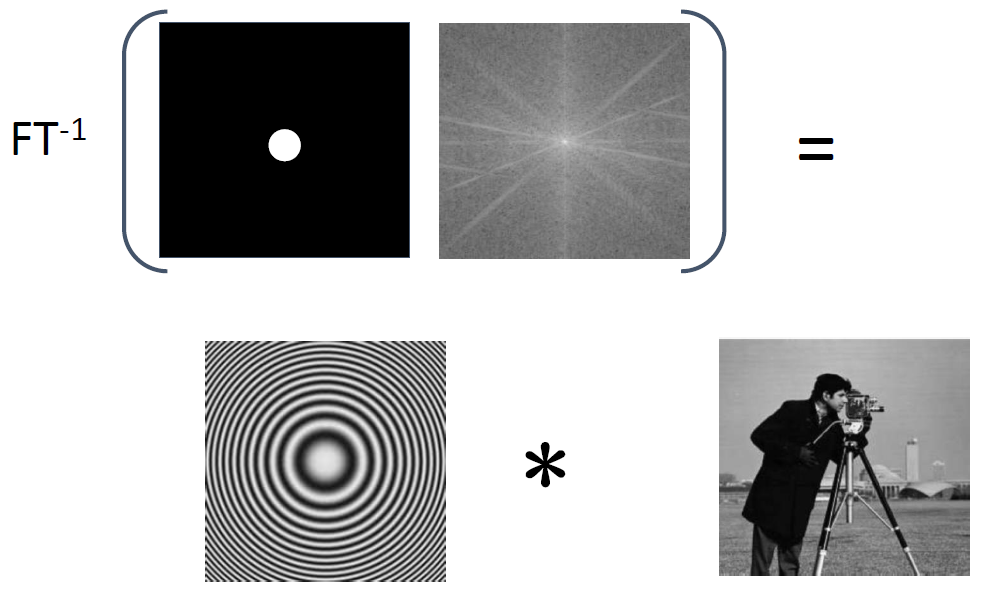
\includegraphics[width=\textwidth]{images/art3.png}
\end{figure}
为了解决这种问题可以使用更为圆滑的Gaussian filters。

\newpage
\subsection{Gaussian Low Pass Filter}
\begin{figure}[bht!]
  \centering
  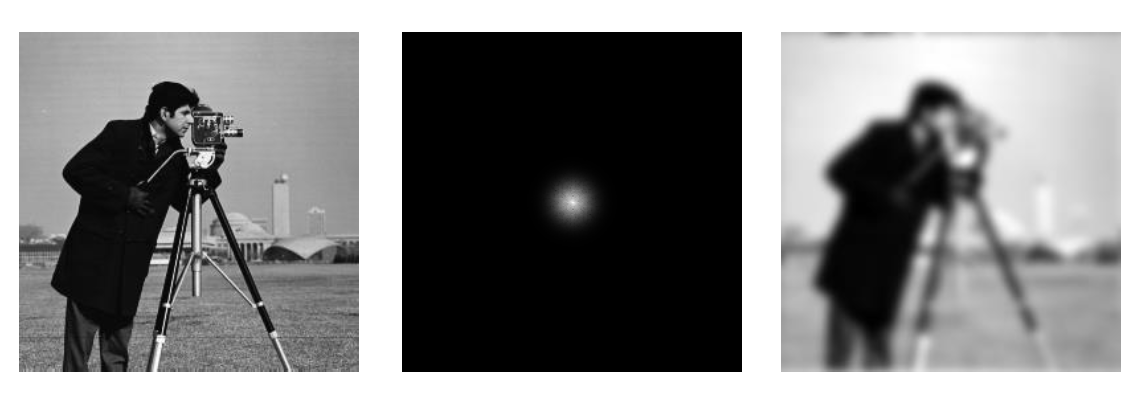
\includegraphics[width=\textwidth]{images/glp.png}
\end{figure}

\subsection{Gaussian High Pass Filter}
\begin{figure}[bht!]
  \centering
  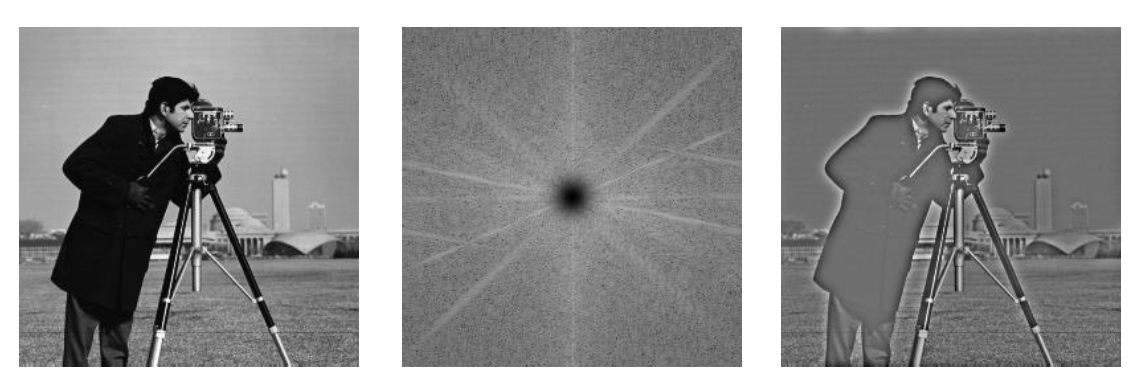
\includegraphics[width=\textwidth]{images/ghp.png}
\end{figure}



\section{Applications}
\begin{itemize}
  \item Image compression 图像压缩
        \begin{itemize}
          \item Human visual system is not very sensitive to contrast in high spatial frequencies
          \item Discarding information in high spatial frequencies doesn’t change the “look” of an image
        \end{itemize}
  \item Image forensics 图像取证
  \item Texture \& scene representation
  \item Shape representation
\end{itemize}




\end{document}
